\documentclass[../templatetop.tex]{subfiles}

\swd{contents/02_literature_review}

\begin{document}

\section{Position estimation using parameters}

After estimating a  set of parameters form the received signals by one of techniques described in the previous section, the next step is to estimate the position from the obtained parameters.
Position estimation techniques can be divide into two category depending on the presence of a database that contain the signal measurements at known positions. A techniques that makes use of such a database which is usually obtain by training phase (off-line phase) before the real time positioning start, is called mapping (fingerprinting) technique. Other techniques that do not utilize such a database commonly employ \textit{geometric} and \textit{statistical} techniques to estimate the position using only parameters estimates form the first step.

\noindent In the absence of a database consisting of previous taken measurements at known positions, the position of the target node should be estimated directly from the available measurements obtained in the first step. Such position techniques can be considered in two groups, geometric and statistic techniques.

\subsection{Mapping techniques}
Mapping techniques use the available database in the system as training data and estimate the position of a target node by pattern-matching algorithms, such as \textit{K-nearest-neighbor (k-NN)}, \textit{support vector regression (SVR)} and \textit{neural networks}.

A mapping technique can be consider as a regression scheme that maps the input vector to an output vector by using a training set. Let the training set be represented by:
\begin{equation}
    \tau = \{(m_1, p_1), (m_1, p_1),..., (m_{N_t}, p_{N_t})\}
\end{equation}
where $m_i$ represents the measurement vector for $i$th position $p_i$ ($p_i=\begin{bmatrix} x_i & y_i \end{bmatrix}^T$ for two-dimensional positioning) and $N_t$ is the total number of training set (the size of the database). For

One of the simplest regression techniques is to estimate the position of the target node as the position vector in the training set $\tau$ corresponding to the measurement vector that has the shortest distance to the measurement vector $m$. In other words, the position is estimated as $p_j$, with:
\begin{equation}
    j = \argmin_{i \in \{1,..,N_t\}} \lVert m - m_i \rVert
\end{equation}
where $\lVert m - m_i \rVert$ represents the Euclidean distance between $m$ and $m_i$.

\subsection{Geometric approach}

A geometric positioning technique solve for the position of the target node as intersection of position lines obtained from set of measurements at a number if reference nodes. For example, the RSS and TOA give us an uncertainty in the shape of a circle while the A0A give us an uncertainty in the shape of a line. In geometric approach, the position of the target node is determined by the intersection of uncertainty regions computed on several nodes.

In case of RSS or TOA, we need to know the distance of target node and three source nodes with known position, $d_i$, as shown in figure \ref{fig:rss_toa_position_model}.

\begin{figure}[htbp]
    \centering
    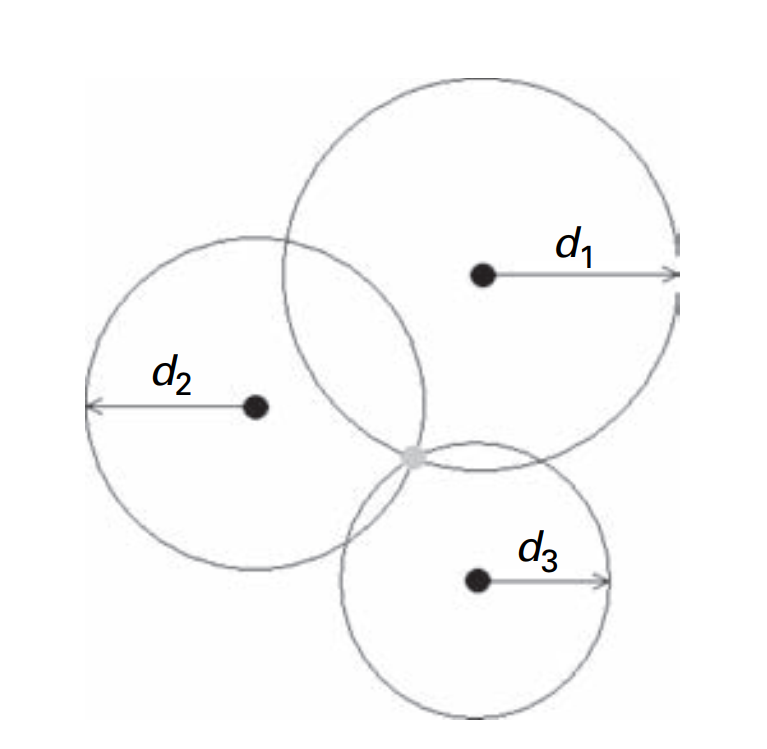
\includegraphics[width=0.5\textwidth]{rss_toa_position_model}
    \caption{The reference (black) nodes measure their distances (via RSS or TOA estimation) from the target node (gray node), which results in three circles passing through the target node. The intersection of the three circles can be calculated to obtain the position of the target node, which is called trilateration}
    \label{fig:rss_toa_position_model}
\end{figure}

Let $d_1$, $d_2$, $d_3$ represent the range measurement obtained from three TOA and RSS measurements. Then, the following system of equations is solved in order to estimate the position of the target node via trilateration:
\begin{equation}
    d_i = \sqrt{(x_i -x)^2 + (y_i - y)^2}  \mbox{,i = 1,2,3}
    \label{eq:rss_toa_system_of_equations}
\end{equation}
where $(x_i, y_i)$ is the known position of the $i$th reference node, and $(x,y)$ is the position of the target node.
The position $(x,y)$ can be solved from \ref{eq:rss_toa_system_of_equations} as:
\begin{equation}
    x = \frac{(y_2-y_1)\gamma_1 + (y_2-y_3)\gamma_2}{2[(x_2-x_3)(y_2-y_1) + (x_1-x_2)(y_2-y_3)]}
\end{equation}
\begin{equation}
    y = \frac{(x_2-x_1)\gamma_1 + (x_2-x_3)\gamma_2}{2[(x_2-x_1)(y_2-y_3) + (x_2-x_3)(y_1-y_2)]}
\end{equation}
where
\begin{equation}
    \gamma_1 = x_2^2 - x_3^2 + y_2^2 - y_3^2 + d_3^2 - d_2^2;
\end{equation}
\begin{equation}
    \gamma_2 = x_1^2 - x_2^2 + y_1^2 - y_2^2 + d_2^2 - d_1^2;
\end{equation}

Using the AOA approach, we need only two source nodes (antenna arrays) to estimate the position of the target node. As depicted in figure \ref{fig:aoa_position_model}, each AOA gives us an uncertainty in the shape of a line; so, we can estimate the target node's position as the intersection of these two lines.

\begin{figure}[htbp]
    \centering
    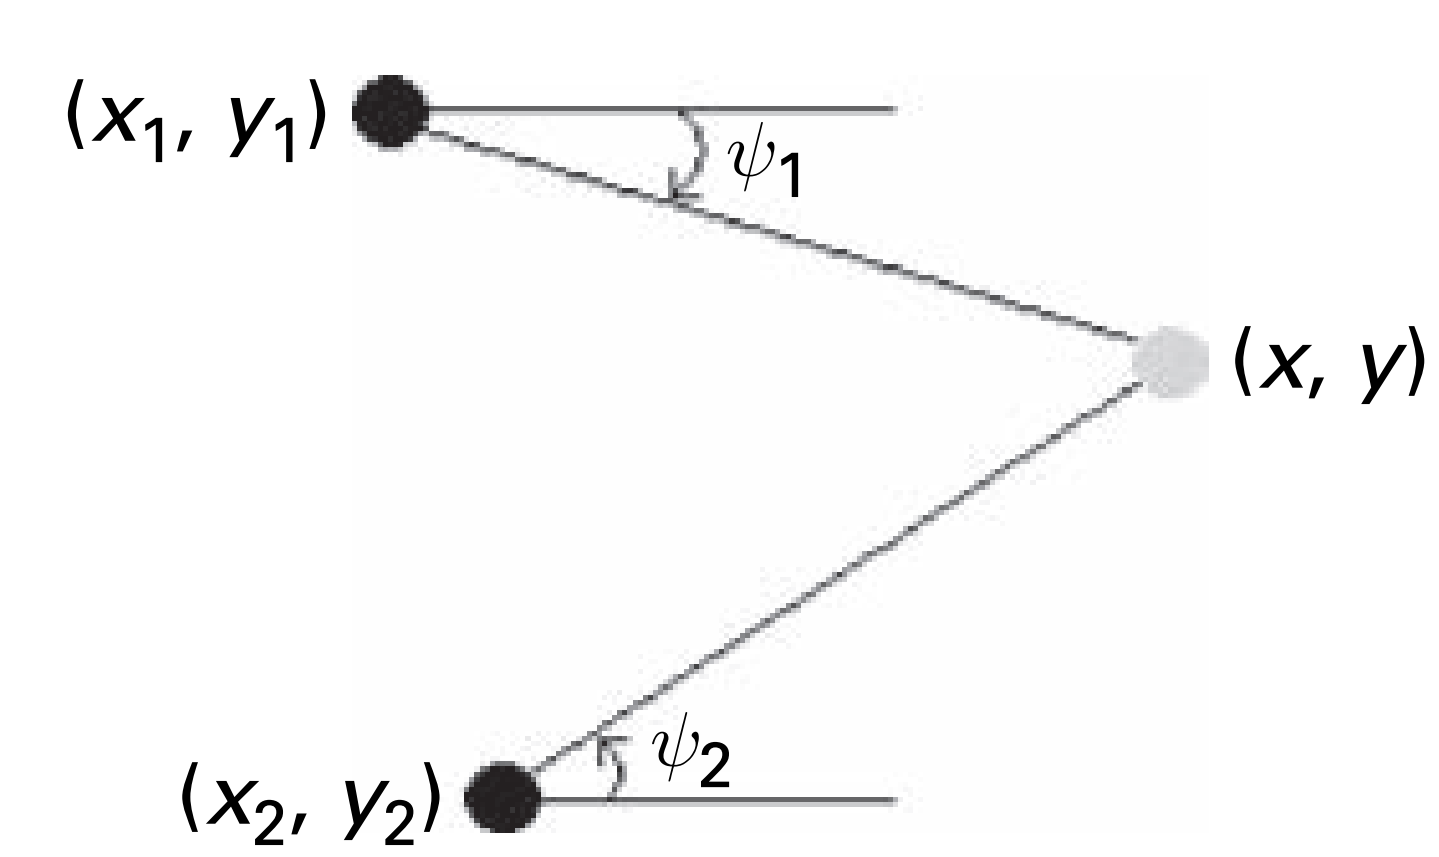
\includegraphics[width=0.5\textwidth]{aoa_position_model}
    \caption{The angles measured by the reference (black) nodes determine two lines, the intersection of
    which yields the target position. This technique is called triangulation}
    \label{fig:aoa_position_model}
\end{figure}

Each line give us an equation like:
\begin{equation}
    \tan{\psi} = \frac{y-y_1}{x-x_1}, i = 1,2
\end{equation}
Solving the equation jointly, we have:
\begin{equation}
    x = \frac{x_2\tan{\psi_2} - x_1\tan{\psi_1} + y_1 - y_2}{\tan{\psi_2} - \tan{\psi_1}}
\end{equation}
\begin{equation}
    y = \frac{(x_2-x_1)\tan{\psi_2}\tan{\psi_1} + y_1\tan{\psi_2} - y_2\tan{\psi_1}}{\tan{\psi_2}-\tan{\psi_1}}
\end{equation}

In case of the TDOA, we need three source nodes with known positions to obtain two TDOAs. As explained in previous section, TDOA is time difference of arrival of transmitted signals from the target node, between two source nodes. On TDOA gives us an uncertainty region in the shape of a hyperbola.

\begin{figure}[htbp]
    \centering
    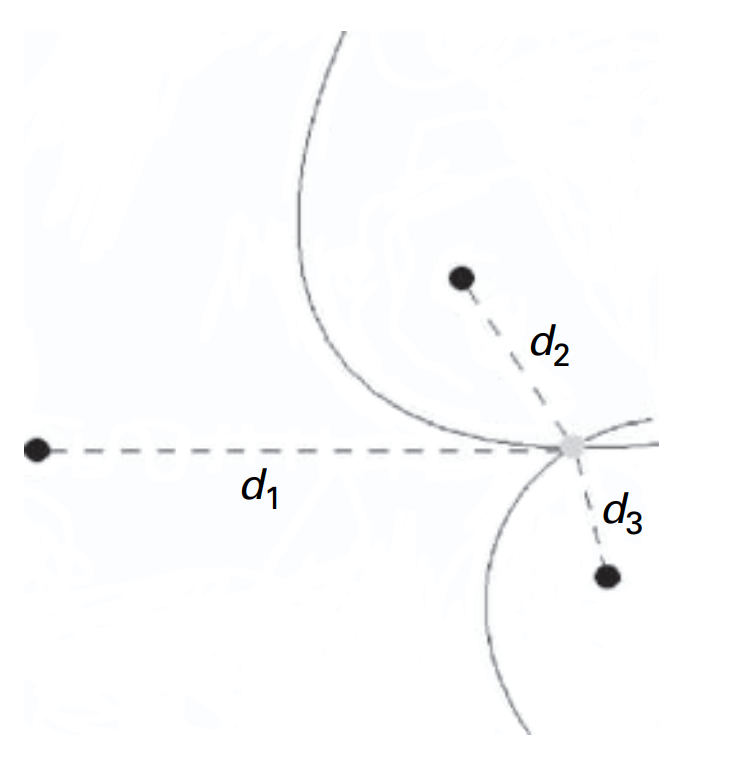
\includegraphics[width=0.5\textwidth]{tdoa_position_model}
    \caption{Each TDOA determines a hyperbola. The position of the target node is estimated by intersection of these two hyperbola}
    \label{fig:tdoa_position_model}
\end{figure}

The hyperbola region is described by the following equation:
\begin{equation}
    d_{i1} = d_i - d_1 = \sqrt{(x-x_i)^2 - (y-y_i)^2} - \sqrt{(x-x_1)^2+(y-y_1)^2}, i =2,3
    \label{eq:tdoa_position_model}
\end{equation}
where
\begin{equation}
    d_1 = \sqrt{(x-x_1)^2 - (y-y_1)^2}
\end{equation}
The position of the target node is estimated by solving the two equations of \ref{eq:tdoa_position_model} jointly.

Since geometric approaches cannot cope with practical noisy eviroments, usually statistical approaches are used in practice. In this noisy framework, we define a model for noisy measurement as:

\section{Statistic approach}
Since geometric approaches cannot cope with noisy environments, usually statistical approach are used in practice. In this noisy framework, we define a model for noisy measurement as:
\begin{equation}
    z = f(x,y) + \eta
\end{equation}
where $z$ is the results of a noisy measurement, $f(x,y)$ is the true value of this measurement which is the function of target node's position and $\eta$ is the noise of this measurement. For the techniques discussed in previous section, $f(x,y)$ is as follows:
\begin{equation}
    f(x,y) = \begin{cases} \sqrt{(x-x_s)^2 + (y-y_s)^2} & \mbox{TOA, RSS} 
    \\ \arctan{\frac{y-y_s}{x-y_s}} & \mbox{AOA}
    \\ \sqrt{(x-x_s)^2 + (y-y_s)^2} - \sqrt{(x-x_{cs})^2 + (y-y_{cs}^2)} & \mbox{TDOA}
\end{cases}
\end{equation}
where $(x_s,y_s)$ is the known position of the source nodes, and $(x_{cs},y_{cs})$ is the position of common source node for the TDOA technique. In vector-space notation, the cited model is changed to:
\begin{equation}
    \mathbf{z} = \mathbf{f}(x,y) + \mathbf{\eta}
\end{equation}
where $\mathbf{z} = [z_1,...,z_{N_m}]^T$, $\mathbf{F}(x,y) = [f_1(x,y),...,f_{N_m}(x,y)]^T$ and $\mathbf{\eta}=[\eta_1,...,\eta_{N_m}]^T$. $N_m$ equal to the number if source node in TOA, RSS amd AOA approaches, and one less than the number of source nodes in the TDOA approach. Assume that the noise which affects our measurements is known except for a set of parameters, $\lambda$. So, we have a vector of unknown parameters, $\theta$, as:
\begin{equation}
    \mathbf{\theta} = [xy\mathbf{\lambda}^T]^T
\end{equation}
where $(x,y)$ is the position of the target node. In such problems, we can use parametric approaches to estimate the  true value of $\mathbf{\theta}$. Two prevalent parametric approaches are Bayesian and Maximum-Likelihood (ML). The Bayesian approach is usefull in case of prior information about $\mathbf{\theta}$ is available. The ML approach find $\mathbf{\theta}$ which gives the maximum probability for the observations. Formally, we can define $\mathbf{\theta}$ estimated by the ML $\hat{\mathbf{\theta}}$ as:
\begin{equation}
    \hat{\mathbf{\theta}}_{ML} = \argmax_{\theta}p(\mathbf{z}|\mathbf{\theta})
\end{equation}
Since the function of $f(x,y)$ is deterministic, we can express the likelihood function $p(\mathbf{z}|\mathbf{\theta})$ as:
\begin{equation}
    p(\mathbf{z}|\mathbf{\theta}) = p_{\eta}(\mathbf{z} - \mathbf{f}(x,y) | \mathbf{\theta}) 
    \label{eq:probability_density_function_of_the_noise}
\end{equation}
where $p(.|\mathbf{\theta})$ is the conditional probability density function of the noise given parameter vector $\mathbf{\theta}$.
\subsubsection*{Position in the presence of the independent noise}
In case of the independent noise for all measurement, we can express equation \ref{eq:probability_density_function_of_the_noise} as:
\begin{equation}
    p(\mathbf{z}|\mathbf{\theta}) = \prod_{i=1}^{N_m}p_{\eta_i}(z_i-f_i(x,y) | \mathbf{\theta})
\end{equation}
where $z_i$ is the $i$th measurement, $f_i(x,y)$ is the true value of the $i$th measurement and the $p_{\eta_i}$ is the conditional probability function of the $i$th measurement. The independent noise assumption is reasonable for the AOA, TOA and RSS approaches. However, in the case of TDOA, we have correlated noise for several source node's measurements due to the presence of the common source node. For system working under LOS conditions, the majority of the noise is thermal noise. We can model the noise of the environments as Gaussian zero mean random variable as:
\begin{equation}
    p_{\eta_i} = \frac{1}{\sqrt{2\pi}\sigma_i}\exp{-\frac{u^2}{2\sigma_i^2}}
\end{equation}
\end{document}